\section{洛伦兹力与速度的关系}
对一个运动电荷，磁力为 $\bm F_B=q\bm v\times\bm B$。电荷量 $q$ 应保留正负；若题目把 $q$ 定义为电量的大小，则电子的实际电荷应写成 $-q$。先按正电荷作叉乘，再依据电荷符号决定是否反向，比混用多种手势更不容易出错。


安培力与单粒子磁力之间可以通过电流联系。横截面积 $A$ 的导体中，载流子数密度为 $n$、漂移速度为 $\bm v_d$，有 $\bm J=nq\bm v_d$。长度 $\Delta l$ 中含 $nA\Delta l$ 个载流子，合磁力为这些载流子的磁力之和，得到 $I\Delta\bm l\times\bm B$。宏观导体的整体速度与载流子相对导体的漂移速度并不相同，讨论机械功时尤其应分清。


单个电荷磁力的功率恒为 $q(\bm v\times\bm B)\cdot\bm v=0$。所以只有静磁场作用时，动能与速率保持不变；方向则可以持续改变。通电导体的安培力能对导体整体运动作功，能量由维持电流的装置及内部电场传递，不能把宏观速度直接替代每个载流子的总速度而制造矛盾。

\fig{fig:mg3:k:lorentz}{磁力与瞬时速度垂直}{\begin{tikzpicture}[scale=.88]
\fill(0,0)circle(3pt)node[left]{$q>0$};\draw[flow](0,0)--(2,0)node[right]{$\bm v$};\draw[force](0,0)--(0,-1.8)node[below]{$q\bm v\times\bm B$};\node at(2,1.2){$\odot B$};
\end{tikzpicture}}

图\ref{fig:mg3:k:lorentz}中的磁力垂直瞬时速度，故点积功率 $q(\bm v\times\bm B)\cdot\bm v$为零。它仍能持续改变速度方向，所以速率不变并不意味着合力为零；电荷变号后力方向相反，轨迹弯曲方向也须随之改变。


\section{匀强磁场中的圆周与螺旋运动}
把速度分解为平行与垂直磁场的两部分。平行分量不受磁力，保持匀速；垂直分量受大小恒定、始终与其垂直的力，作圆周运动。非相对论条件下，
\begin{equation}r=\frac{mv_\perp}{|q|B},\qquad
\Omega=\frac{|q|B}{m},\qquad T=\frac{2\pi}{\Omega},\qquad
p_z=v_\parallel T.\end{equation}
这里 $v_\parallel$ 取沿磁场方向的有向分量，$p_z$ 是一周的有向轴向推进；若螺距表示长度，则 $p=|p_z|$。下文图示取 $v_\parallel>0$，其推进长度与几何螺距相等。
圆周周期不依赖速率与轨道半径，是回旋加速和磁聚焦的基础。它依赖质荷比 $m/|q|$，因此不同粒子的周期一般不同。这里忽略辐射损失，并要求速度远小于光速；高能情况下动量与速度的关系需要改变。


作平面轨道时，圆心位于瞬时磁力指向的一侧，距离为 $r$。更一般地，在均匀场中垂直平面的圆心位置可写成 $\bm r_c=\bm r+\frac{m}{qB^2}\bm v\times\bm B$。这给出了带符号的圆心定位，避免把负电荷的轨道画向相反侧。


例如 $q>0$、磁场向纸内，粒子从原点以 $v_0$ 沿 $+x$ 入射，圆心为 $(0,r)$。将 $\bm B=-B\bm e_z$ 代入牛顿定律，
\[
 \dot v_x=-\Omega v_y,\qquad \dot v_y=\Omega v_x,\qquad
 \Omega=qB/m>0.
\]
这里 $\Omega$ 为常量。对第一式求导，代入第二式，
\[
 \ddot v_x=-\Omega\dot v_y=-\Omega(\Omega v_x)=-\Omega^2v_x.
\]
试取 $v_x=e^{st}$，则 $\dot v_x=se^{st}$、$\ddot v_x=s^2e^{st}$。
代回得 $(s^2+\Omega^2)e^{st}=0$，故特征根为 $s=\pm\mathrm i\Omega$。
实通解及其导数为
\[
 v_x=A\cos\Omega t+D\sin\Omega t,\qquad
 \dot v_x=-A\Omega\sin\Omega t+D\Omega\cos\Omega t.
\]
由 $v_x(0)=v_0$ 得 $A=v_0$，由 $\dot v_x(0)=-\Omega v_y(0)=0$ 得 $D\Omega=0$，即 $D=0$。
再用 $v_y=-\dot v_x/\Omega$，得到 $v_y=v_0\sin\Omega t$。
位置从初始原点积分：
\[
 x=v_0\int_0^t\cos\Omega s\dd s
   =\frac{v_0}{\Omega}[\sin\Omega s]_0^t,\qquad
 y=v_0\int_0^t\sin\Omega s\dd s
   =-\frac{v_0}{\Omega}[\cos\Omega s]_0^t.
\]
因 $v_0/\Omega=r$，用速度转角 $\phi=\Omega t$ 表示，

\[
v_x=v_0\cos\phi,\quad v_y=v_0\sin\phi,\qquad
x=r\sin\phi,\quad y=r(1-\cos\phi).
\]
坐标参数式既给圆的方程，也保留沿轨道行进的先后顺序。只写圆方程会丢失运动方向与首次到达时刻，处理边界问题时尤其不够。
\fig{fig:mg3:k:orbit}{以向心力定位圆心，实际转角同时决定位置与速度方向}{\begin{tikzpicture}

\draw[axis](-.4,0)--(3,0)node[right]{$x$};\draw[axis](0,-.3)--(0,3.3)node[above]{$y$};
\draw[->,blue,thick](0,0)arc(-90:30:1.4);\fill(0,1.4)circle(1.6pt)node[left]{$C(0,r)$};\fill(0,0)circle(1.6pt)node[below left]{$O$};\fill(1.212436,2.1)circle(1.6pt)node[right]{$P$};
\draw[flow](0,0)--(1,0)node[below]{$v_0$};\draw[force](0,0)--(0,.85)node[left]{$F_B$};\draw[guide](0,0)--(0,1.4)--(1.212436,2.1);
\draw[dim](0,.9)arc(-90:30:.5);\node at(.7,1.08){$\phi$};\draw[flow](1.212436,2.1)--(.712436,2.966025)node[above]{$\bm v(t)$};\node at(2.8,2.6){$\otimes B,\ q>0$};

\end{tikzpicture}}

图\ref{fig:mg3:k:orbit}先从入射速度与磁场判断向心力，再沿该法线定位圆心。飞行时间对应实际扫过的圆心角，不能把入射、出射速度的锐夹角无条件当作全部转角；超过半周或经过多次边界时，应沿真实运动方向逐段计角。


\section{有限磁区与首次出界}
磁场被边界截断后，粒子只在磁区内部沿圆弧运动，离开后沿出界时的切线作直线运动。解题顺序是定位圆心、求几何交点，再按参数角判断哪个交点先被到达。圆周与直线往往有两个交点，其中一个可能就是入射点，另一个也未必处于题目允许的边界段。


求时间可用 $t=\Delta\phi/\Omega$，其中 $\Delta\phi$ 必须是沿实际转动方向扫过的角度。由一个正弦值反求角度时，需要结合速度方向选择象限；不能仅把计算器给出的锐角当作全部运动时间。相切也不总等于穿出：若圆弧在边界处只有一个接触点，前后仍都位于磁区内，粒子并未进入区外。


处理两种不同磁场组成的分区时，位置、速度在无冲量边界上连续，速率不变，但圆心与曲率立即改变。每次过界都应以当时的速度重新定位下一圆心，不能让两段半径不同的弧共用同一个圆心。重复过界问题可以先找一个完整周期的位移与时间，再累计；平均速度由总位移除以总时间给出，不能平均两个回旋速度的大小。


\fig{fv:m3:exit}{圆轨迹只是候选延拓，物理轨迹在首次有效出界处切换}{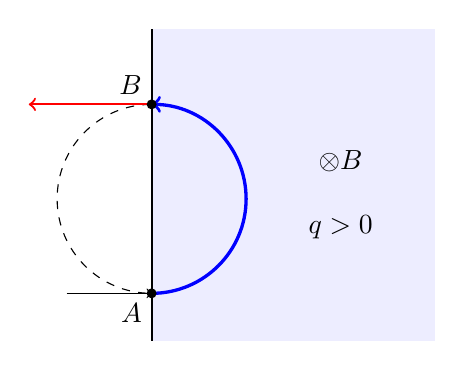
\begin{tikzpicture}[scale=1.2]
\fill[blue!7](1,-.5)rectangle(4,2.8);\draw[thick](1,-.5)--(1,2.8);\draw[dashed](1,1)circle(1);
\draw[->,blue,very thick](1,0)arc(-90:90:1);\draw[->,red,thick](1,2)--(-.3,2);
\draw[->](.1,0)--(1,0);\fill(1,0)circle(1.5pt)node[below left]{$A$};\fill(1,2)circle(1.5pt)node[above left]{$B$};
\node at(3,1.4){$\otimes B$};\node at(3,.7){$q>0$};\end{tikzpicture}}
图\ref{fv:m3:exit}中正电荷由 $A$向右进入磁场，洛伦兹力最初向上，圆心在入射点正上方。只有右半圆处于磁区，第一次回到边界的 $B$才是出界事件；此后沿切线直飞，不能继续沿虚线圆周运动。求有限磁区题时，先由入射位置和力方向定圆心，再按转动方向排列各边界交点；最小正飞行时间对应的有效交点才能连接下一阶段。


\section{磁区边缘的连续条件}
理想磁区边缘把场从一个有限值改成另一个有限值。只要磁感应强度没有狄拉克脉冲式奇异，粒子穿过宽度趋零的边缘层时，所受冲量 $\int q\bm v\times\bm B\dd t$ 也趋零。因此位置和速度都连续，轨迹在边界处具有同一条切线；发生突变的是加速度与曲率，而不是速度方向本身。


将两段圆弧拼接时，应先确定入界点，再把该点处的速度方向作为新圆的切线。第二圆心落在切线的法线上，其哪一侧由电荷正负与磁场方向决定，圆心距离则由新的 $r=mv/(|q|B)$ 决定。这个步骤不能用“半径变了，所以折射角改变”替代。光线折射允许界面处方向发生转折，这里的有限磁力没有提供瞬时转向所需的冲量。


真实磁区边缘存在漏磁和渐变区域。若渐变层厚度 $\delta$ 远小于轨道半径，理想锐边模型可近似计算整体偏转；若研究的是绝热不变量，反而要求场在一个回旋尺度内变化缓慢。两种近似服务于不同问题，不宜在同一个锐边处一面使用突然拼圆，一面又声称磁矩严格守恒。


边界还需满足磁场无源条件。此处常画的纸面内分界线对应 $\bm B$ 垂直纸面，因而磁场平行于真实界面，允许切向分量跳变。若把磁场设为垂直界面的方向，则其法向分量不能在界面两侧任意从有限值跳成零，必须进一步考虑三维漏磁结构。

\fig{fig:mg3:k:join}{过界时共用同一切线，再按新半径另定圆心；图示 $B_2=2B_1$}{\begin{tikzpicture}

\fill[blue!7](-2.8,-.4)rectangle(0,3);\fill[orange!10](0,-.4)rectangle(2.8,3);\draw[world](0,-.5)--(0,3.1);
\draw[->,blue,thick](-1.532089,.714425)arc(-140:-90:2);\draw[->,red,thick](0,0)arc(-90:0:1);
\fill(0,0)circle(1.6pt)node[below left]{$P$};\fill(0,2)circle(1.6pt)node[left]{$C_1$};\fill(0,1)circle(1.6pt)node[right]{$C_2$};
\draw[flow](0,0)--(1.4,0)node[below]{$\bm v_P$};\draw[dim](-.5,0)--(-.5,2)node[midway,left]{$r_1$};\draw[dim](.5,0)--(.5,1)node[midway,right]{$r_2$};
\node at(-1.8,2.65){$\otimes B_1$};\node at(1.8,2.65){$\otimes B_2$};\node at(0,-1.2){切线与速率连续，$r_1/r_2=B_2/B_1$};

\end{tikzpicture}}
图\ref{fig:mg3:k:join}中，两段轨道在 $P$ 点的速度都向右，两圆心因而都在穿过 $P$ 的竖直法线上。两区磁场同向，圆心也在同一侧；第二段的场更强、圆心更近。若磁场反向，第二圆心应换到法线的另一侧，但粒子仍先以原来的向右速度进入新区。连续的是速度，改变的是随后的偏转率。



\section{由轨迹反求圆心与磁区参数}
已知轨迹上一点和该点速度，只能确定圆心所在直线，还不能确定圆心位置。再给定另一个点，利用两点连线的中垂线，才能求出候选圆心。若两个点的切线都给定，则两条法线交点提供圆心，并可检验它到两点的距离是否相等。没有通过这个等距检验的图形，不能用来建立同一个匀强场圆轨道。


几何条件可能同时给出多个圆或多条圆弧。必须进一步选择符合电荷转向、首次出界、运动方向和可达区域的分支。圆与边界有两个交点时，粒子从入点开始沿实际转向走到的第一个交点才是出点；不能为了得到较短公式而任意取另一个交点。若先撞到其他边界，后面的交点即使满足圆方程也不属于实际过程。


对最小磁区问题，仅构造一个能够包含轨迹的圆通常只能证明上界。还要给出下界，例如用轨迹两端点间弦长说明覆盖圆半径至少为弦长的一半，再证明达到该下界的圆确实包含整段实际圆弧。若还限制磁区必须处于某象限或不能接触发射器，就要验证圆盘边界同样满足这些限制。最小值、下确界和可达到的临界情形应分开表述。

\fig{fig:mg3:k:inverse}{圆心由切线法线与弦的中垂线共同确定}{\begin{tikzpicture}[scale=.88]
\draw[world](0,0)arc(-90:0:2);\fill(0,0)circle(2pt)node[below]{$P$};\fill(2,2)circle(2pt)node[right]{$Q$};\draw[flow](-1,0)--(.7,0)node[below]{$v_P$};\draw[flow](2,2)--(2,3)node[above]{$v_Q$};\draw[guide](0,0)--(0,2)node[above]{$C$}--(2,2);\draw[guide](0,0)--(2,2);\draw[guide](.3,1.7)--(1.7,.3)node[right]{中垂线};
\end{tikzpicture}}

图\ref{fig:mg3:k:inverse}的圆心同时位于入射切线的法线上和进出点连线的中垂线上，两条几何条件共同确定半径。求出圆心后还要用电荷符号及磁场方向筛选运动弧段，单凭两个端点并不能确定实际转动方向。


\section{限定磁区大小的几何下界}
若要求用一个圆形磁区使速度方向改变给定角度，磁区必须包含实际运动圆弧。对不超过半周的圆弧，弦长为 $2r\sin(\Delta\phi/2)$，任何覆盖两个端点的圆盘半径至少是弦长的一半。以弦为直径作圆盘，还需证明整段圆弧确实在盘内，才能把下界当作可达最小值。


当圆弧超过半周时，端点距离可能重新变小，仅用端点就会严重低估磁区。因为弧中已经包含轨道圆的某一对对径点，覆盖圆盘至少要有半径 $r$。最小区域题的关键因此包括两个部分：从几何上得到不可再小的下界，并构造满足入、出射方向且能覆盖整个路径的磁区。


同样，等边三角形磁区的边长不可能小于两弧端点的距离；能否将弦作为三角形的一边，还要检查弧位于三角形内、直线进出段不会提前再穿入磁区，以及三角形能否放进题目给定的大区域。构造图中的每一个条件都对应一个可实现性检查，不能只画出一个小图形就结束。

\fig{fig:mg3:k:cover}{小于半周的圆弧可由弦的直径圆覆盖；必须同时检查直线进出段}{\begin{tikzpicture}

\filldraw[fill=blue!7,draw=blue](1,0)circle(1.732051);\draw[guide](0,0)circle(2);\draw[->,red,very thick](1,-1.732051)arc(-60:60:2);
\fill(0,0)circle(1.5pt)node[left]{$C$};\fill(1,0)circle(1.5pt)node[below]{$M$};\fill(1,-1.732051)circle(1.5pt)node[below]{$P$};\fill(1,1.732051)circle(1.5pt)node[above]{$Q$};
\draw[guide](0,0)--(1,-1.732051);\node[left]at(.4,-.8){$r$};\draw[guide](1,-1.732051)--(2.9,-1.732051)(1,1.732051)--(2.9,1.732051);\draw[dim](2.9,-1.732051)--(2.9,1.732051)node[midway,right]{$2R_{\min}$};
\draw[flow](.133975,-2.232051)--(1,-1.732051);\draw[flow](1,1.732051)--(.133975,2.232051);
\node[align=center]at(5.6,1.1){轨道圆心 $C$\\覆盖圆心 $M$\\$R_{\min}=r\sin(\Delta\phi/2)$};\node at(1,-3){图示 $\Delta\phi=2\pi/3$，红弧位于蓝色圆盘内};

\end{tikzpicture}}
图\ref{fig:mg3:k:cover}中 $M$ 是弦中点。以轨道圆心为原点、弦中点位于正横轴，记 $\eta=\Delta\phi/2<\pi/2$，任意弧点 $X$ 可写为 $(r\cos u,r\sin u)$，$|u|\le\eta$。它到 $M=(r\cos\eta,0)$ 的距离满足

\[
 |XM|^2=r^2(1+\cos^2\eta-2\cos\eta\cos u)
 \le r^2\sin^2\eta.
\]
因此整段短弧确实在弦的直径圆内，端点达到半径下界。这里不等式中的距离指任意弧点到 $M$，不能只检查两个端点。对严格小于半周的转角，图中直线进入、离开覆盖圆的方向也分别指向盘内、盘外。


还须区分几何覆盖与真实进出磁区。若允许弧落在边界上，半周及更长弧的几何最小覆盖半径为 $r$；若要求实际磁轨道处于磁区内部并在两端穿越边界，半径恰为 $r$ 的同心圆会让轨道沿边界运行，不能直接作为可实现的进出过程。这时要检查边界的定义；严格内部条件下，$r$ 可能只是可逼近的下确界。练习中的覆盖问题已明确允许落在圆盘边界上。



\section{回旋加速、磁分析与聚焦}
回旋加速器在磁场内使粒子转过半周，再在间隙内用电场增加动能；磁场自身不做功。理想非相对论回旋周期固定，交流电压可按同一周期同步。每次跨缝增加 $qU$，一整圈跨缝两次，因此整圈增加 $2qU$。最大半径决定可容纳的最大动量，从而决定最大动能，不能把“周期固定”误解为速度不变。


\fig{fig:mg3:k:cyclotron}{D形盒内由磁场转向，跨缝时由电场加速；缝宽已放大表示}{\begin{tikzpicture}

\draw[world](.15,2.7)arc(90:-90:2.7)--cycle;\draw[world](-.15,2.7)arc(90:270:2.7)--cycle;
\draw[->,blue,thick](.15,0)arc(-90:90:.7);\draw[blue,thick](.15,1.4)--(-.15,1.4);\draw[->,orange!80!black,thick](-.15,1.4)arc(90:270:1.1);\draw[orange!80!black,thick](-.15,-.8)--(.15,-.8);\draw[->,red,thick](.15,-.8)arc(-90:90:1.5);
\node at(1.8,-1.8){$\otimes B$};\node at(-1.6,-1.8){$\otimes B$};\node[right]at(3,1.4){每次跨缝 $\Delta K=qU$};\node[right]at(3,.5){每圈跨缝两次};
\node at(0,3.35){交变缝电场与半周飞行时间同步};\node at(0,-3.4){$T=2\pi m/(qB)$，$r$ 随动量增加而增大};

\end{tikzpicture}}
图\ref{fig:mg3:k:cyclotron}中的三段半圆按先右、再左、再右的次序连接。跨缝后的速率增大，下一段轨道半径随之增大，但理想半周时间仍为 $\pi m/(qB)$。交流电场每半周期换向，使粒子在相反方向跨缝时仍被加速；这将恒定磁周期与逐次增长的动能联系起来。




磁分析把轨道半径或落点与质荷比联系。若粒子先经电势差 $U$ 从静止加速，则 $\tfrac12mv^2=|q|U$，再代入回旋半径，得到 $r=\sqrt{2mU/|q|}/B$。这时半径随质量的平方根变化；若先用速度选择器使各粒子速度相同，半径则与质量成正比。所比较的是不同的入射准备条件。


\fig{fig:mg3:k:analyzer}{先由电压准备入射速率，再由半周磁偏转把质量差转成落点差}{\begin{tikzpicture}

\fill[blue!7](0,-.5)rectangle(3.7,3.5);\draw[world](0,-.5)--(0,3.5);\draw[->,blue,thick](0,0)arc(-90:90:1.4);\node at(2.8,2.5){$\otimes B$};
\draw[world](-3.2,-.6)--(-3.2,-.12)(-3.2,.12)--(-3.2,.6)(-1.2,-.6)--(-1.2,-.12)(-1.2,.12)--(-1.2,.6);\draw[flow](-3.7,0)--(-.1,0)node[midway,above]{$v$};\node at(-2.2,-1.1){加速电势差 $U$};
\fill(0,0)circle(1.5pt)node[below left]{入口};\fill(0,2.8)circle(1.5pt)node[left]{探测器};\draw[dim](-.7,0)--(-.7,2.8)node[midway,left]{$D=2r$};
\node at(.3,4.1){$|q|U=mv^2/2,\quad r=mv/(|q|B)$};

\end{tikzpicture}}
图\ref{fig:mg3:k:analyzer}在同一电压下给不同质量的粒子相同的动能，并未给它们相同的速率。先按各自质量求 $v$，才得到 $D=2\sqrt{2mU/|q|}/B$。若入口前改成速度选择器而保持 $v$ 相同，便应直接用 $D=2mv/(|q|B)$，质量依赖从平方根变成一次关系。




轴向磁聚焦利用同一质荷比粒子经过一个回旋周期后横向位移回到零。精确的轴向焦距为 $v_\parallel T$；同一总速率但不同入射角的粒子，其平行速度并不完全相同，只有小角近轴条件下才近似同焦。初始角度与速率分散分别造成角向与色散误差，应明确近似是在哪一步使用的。

\fig{fig:mg3:k:helix}{螺旋轨迹的空间投影；辅助椭圆是垂直场的截面，不是另一条运动轨迹}{\begin{tikzpicture}

\draw[axis](-.8,0)--(7.2,0)node[right]{$z,\bm B$};\foreach \z in {0,3,6}{\draw[guide](\z,0)ellipse(.35 and .8);}
\draw[->,blue,thick,domain=0:720,samples=220]plot({\x/120+.35*cos(\x)},{.8*sin(\x)});
\draw[dim](.35,-1.4)--(3.35,-1.4)node[midway,below]{$p=v_\parallel T$};\draw[guide](6,.8)--(6.5,.8);\draw[dim](6.5,0)--(6.5,.8)node[midway,right]{$r$};
\draw[->,red,thick](.35,0)--(1.65,0)node[above]{$v_\parallel$};\draw[->,red,thick](.35,0)--(.35,1.25)node[above]{$v_\perp$};
\node at(3.7,2){$r=mv_\perp/(|q|B)$，同一周期内轴向前进一螺距};

\end{tikzpicture}}

图\ref{fig:mg3:k:helix}把速度分成平行场与垂直场两部分：前者决定每周轴向前进距离，后者决定回旋半径。无电场、均匀静磁场中二者大小分别不变；有向推进来自同一个回旋周期乘有向平行速度，几何螺距取其绝对值，不能改用总速率乘周期。


\section{空间聚焦与时间聚焦的区别}
半平面磁场中，从边界同一点出发、速率相同而入射角略有不同的一束粒子，可以在边界附近再次会聚。设边界为 $x=0$，场位于 $x>0$，正粒子进入时 $\bm v=v(\cos\alpha,\sin\alpha)$，磁场垂直纸面向里。圆心为 $C=(-r\sin\alpha,r\cos\alpha)$，与边界的第二交点为 $Q=(0,2r\cos\alpha)$。


在 $\alpha=0$ 附近，$y_Q=2r-r\alpha^2+O(\alpha^4)$，没有角度的一阶项。这意味着小角度发散造成的落点分散是二阶量，形成空间上的一阶聚焦。但从初始半径到出点半径的实际转角为 $\pi-2\alpha$，飞行时间为 $(\pi-2\alpha)/\Omega$，其中 $\Omega=|q|B/m$。时间差仍然含角度的一阶项，所以空间聚焦不能直接推出等时到达。


对于速率略有不同的粒子，$r$ 随 $v$ 线性变化，即使角度聚焦，落点仍对速度有一阶色散。需要先通过速度选择器限制速度，才能将落点差主要解释为荷质比差。若关心脉冲束到达时间，还需另外计算时间色散，不能仅凭轨迹会聚图判断时间分辨率。

\fig{fig:mg3:k:space-time}{同速而正负入射角不同的两条实际轨迹在同一边界点相交，飞行转角却不同}{\begin{tikzpicture}

\fill[blue!5](0,-.7)rectangle(3.3,3);\draw[world](0,-.7)--(0,3.1);
\draw[->,blue,thick](0,0)arc(-65:65:1.4);\draw[->,red,thick](0,0)arc(-115:115:1.4);
\fill(0,0)circle(1.6pt)node[left]{$O$};\fill(0,2.537662)circle(1.6pt)node[left]{$Q$};\draw[->,blue](0,0)--(.9063,.4226)node[right]{$+\alpha$};\draw[->,red](0,0)--(.9063,-.4226)node[right]{$-\alpha$};
\node[align=center]at(5.7,2.2){相同落点\\$y_Q=2r\cos\alpha$};\node[align=center]at(5.7,.6){蓝：$T_+=(\pi-2\alpha)/\Omega$\\红：$T_-=(\pi+2\alpha)/\Omega$};\node at(3,-1.3){图示 $\alpha=25^\circ$；空间会聚不保证等时到达};

\end{tikzpicture}}
图\ref{fig:mg3:k:space-time}中，蓝弧少于半周，红弧多于半周，但两个出口坐标完全相同。两者时间差为 $4\alpha/\Omega$，对小角度仍是一阶量。相反，落点对 $\alpha$ 的变化以 $\alpha^2$ 开始；求空间分辨率与求到达时间，必须保留不同阶的几何信息。



\section{受约束带电物体与径向条件}
带电物体还受重力、绳力或支持力时，磁力虽然仍不做功，却会改变约束力。应先由能量或竖直平衡确定可确定的量，再在法向列牛顿方程。磁力指向圆心时可以分担向心力，使绳力减小；反向运动时磁力反向，绳力则增大。因此同一条几何轨道的两个运动方向，约束可实现性可能不同。


细绳只能拉、不能推，光滑接触面只能按允许方向提供支持。由圆周运动方程得到一个实根速度，并不保证约束力符号正确；反过来，将判别式设为零寻找临界半径，也必须确认圆锥的内外表面、尖顶方向和法线方向已经规定。


磁摆的能量仍由重力决定。若最大摆角为 $\alpha$，速度满足 $v^2=2gL(\cos\theta-\cos\alpha)$。把它代入径向受力式后，绳力成为速度的二次函数，但速度只在实际摆动允许的有限区间内取值。二次函数的无约束顶点若落在区间外，临界状态就发生在区间端点；这类范围检验是求最大磁场不可省略的一步。

\fig{fig:mg3:k:pendulum}{先由重力确定可达速率区间，再在此区间内检查磁力向内时的最小绳力}{\begin{tikzpicture}

\fill(0,0)circle(1.6pt)node[above]{$O$};\draw[guide](0,0)--(0,-2.8);\draw[world](0,0)--(1.25,-2.165064);\fill(1.25,-2.165064)circle(2pt);
\draw[force,red](1.25,-2.165064)--(.7,-1.212435)node[left]{$T$};\draw[force,blue](1.5,-2.02)--(1,-1.154)node[right]{$qBv$};\draw[force](1.25,-2.165064)--(1.25,-3.5)node[right]{$mg$};\draw[flow](1.1,-2.3)--(.234,-2.8)node[left]{$v$};\node at(-1.2,-1.2){$\odot B$};\node at(.5,-4.2){图示磁力向内的半程};
\begin{scope}[xshift=5cm,yshift=-3.3cm]
\draw[axis](0,0)--(4.4,0)node[right]{$v$};\draw[axis](0,0)--(0,4.7)node[above]{$B_{\rm lim}(v)$};
\draw[blue,thick,domain=.5:1.4,samples=60]plot(\x,{.5*\x+2/\x});\draw[gray,dashed,domain=1.4:4,samples=60]plot(\x,{.5*\x+2/\x});
\draw[guide](1.4,0)--(1.4,2.128571);\node[below]at(1.4,0){$v_{\max}$};\draw[guide](2,0)--(2,2);\node[below]at(2,-.55){$v_c$};\node[align=center]at(2.4,5.4){图示 $v_{\max}<v_c$\\只在蓝色可达区间取最小值};
\end{scope}

\end{tikzpicture}}
图\ref{fig:mg3:k:pendulum}左图选择磁力向内的半程，绳力为 $T=mv^2/L+mg\cos\theta-qBv$。另一半程磁力反向，绳力只会更大。将能量关系代入，得到

\[
 T(v)=\frac{3m}{2L}v^2-qBv+mg\cos\alpha,
 \qquad 0\le v\le v_{\max}=\sqrt{2gL(1-\cos\alpha)}.
\]
对于 $v>0$，$T\ge0$ 等价于 $B\le B_{\rm lim}(v)=[3mv/(2L)+mg\cos\alpha/v]/q$。图中右侧的虚线只是函数的不可达延拓。对速度求导时，将 $1/v$ 写为 $v^{-1}$，有
\[
 \frac{\dd B_{\rm lim}}{\dd v}
 =\frac1q\left[\frac{3m}{2L}-mg\cos\alpha\,v^{-2}\right].
\]
导数在其零点左侧为负、右侧为正，故无约束极小位置 $v_c=\sqrt{2gL\cos\alpha/3}$ 若超过 $v_{\max}$，须取区间右端；只有落入可达区间时，才能取内部极小值。端点 $v=0$ 的绳力为 $mg\cos\alpha>0$，不必用含 $1/v$ 的式子代入。



\section{带电摆完整竖直圆周的约束}
竖直圆周中的磁力不作功，速率仍由重力势能变化决定；但磁力进入径向方程，会改变绳的拉力。取底部速率 $v_b$，以从最低点转过的角度 $\varphi$ 表示位置，则 $v^2=v_b^2-2gL(1-\cos\varphi)$。选择磁力始终指向圆心的转向，径向方程给 $T=mv^2/L+mg\cos\varphi-qBv$。


将 $\cos\varphi=(v^2-v_b^2+2gL)/(2gL)$ 代入，拉力变为 $T=3mv^2/(2L)-qBv+mg-mv_b^2/(2L)$。要求绳不松弛，相当于对实际可达速率区间逐点要求 $B\le(3mv/(2L)+C/v)/q$，其中 $C=mg-mv_b^2/(2L)$。


若无场时已能完成圆周，即 $v_b^2\ge5gL$，则 $C<0$。上述上界关于 $v$ 的导数为 $[3m/(2L)-C/v^2]/q>0$，因而最严格的位置是速率最小的最高点。设 $v_t=\sqrt{v_b^2-4gL}$，临界场为 $B_{\max}=(m/q)(v_t/L-g/v_t)$。这里“最高点最严格”是经过单调性证明的结论，不是任何带电摆都能预先套用的经验；有限摆动和从静止释放的问题具有不同可达区间。


\fig{fig:mg3:k:fullcircle}{完整圆周中，选定的转向使磁力始终向心；最高点处重力也向心}{\begin{tikzpicture}

\draw[world](0,0)circle(2);\fill(0,0)circle(1.5pt)node[below left]{$O$};\fill(0,2)circle(2pt)node[above left]{$Q$};\fill(0,-2)circle(2pt)node[below right]{$P$};
\draw[flow](0,2)--(1.4,2)node[above]{$v_t$};\draw[flow](0,-2)--(-1.4,-2)node[below]{$v_b$};\draw[flow](2,0)arc(0:-65:2);
\draw[force,blue](0,2)--(0,.7)node[right]{$T_t+qBv_t$};\draw[force]( -.16,2)--(-.16,1.1)node[left]{$mg$};
\draw[force,blue](0,-2)--(0,-.7)node[right]{$T_b+qBv_b$};\draw[force](-.16,-2)--(-.16,-3)node[left]{$mg$};
\draw[dim](0,0)--(2,0)node[midway,below]{$L$};\node at(-2.8,.5){$\odot B$};
\node[right,align=center]at(3.1,1.3){最高点：$T_t+qBv_t+mg=mv_t^2/L$\\能量：$v_t^2=v_b^2-4gL$};
\node[right,align=center]at(3.1,-1.1){$T_t\ge0$ 给 $B\le(m/q)(v_t/L-g/v_t)$\\还需用全程单调性检查其他点};

\end{tikzpicture}}
图\ref{fig:mg3:k:fullcircle}中，最高点的重力和磁力都帮助提供向心力，因此在同一顶点速率下，增大向内磁场会减小所需绳力。令 $T_t=0$ 可以给出候选临界场；只有前面已证明最高点对应全程最严格上界，才能把它确定为完整圆周的临界值。若磁力反向或速率可达区间不同，必须重新检查，不能照搬最高点条件。
